%--------------------------------------------------------------------------
%	PACKAGES AND OTHER DOCUMENT CONFIGURATIONS
%--------------------------------------------------------------------------
\documentclass[11pt,a4paper]{article}
\usepackage[utf8]{inputenc}
\usepackage[francais]{babel}
\usepackage[T1]{fontenc}
\usepackage{amsmath}
\usepackage{amsfonts}
\usepackage{amssymb}
\usepackage{graphicx}
\usepackage{lmodern}
\usepackage[left=2cm,right=2cm,top=2.2cm,bottom=2.2cm]{geometry}

\usepackage{fancyhdr} % Required for custom headers
\usepackage{lastpage} % Required to determine the last page for the footer
\usepackage{extramarks} % Required for headers and footers
\usepackage[usenames,dvipsnames]{color} % Required for custom colors
\usepackage{graphicx} % Required to insert images
\usepackage{caption}
\usepackage{subcaption}
\usepackage{listings} % Required for insertion of code
\usepackage{courier} % Required for the courier font
\usepackage{verbatim}
\usepackage{multirow}
\usepackage{eurosym}
\usepackage[squaren,Gray]{SIunits}
\usepackage{url}
\usepackage{hyperref}

% Margins
%\topmargin=-0.45in
%\textwidth=6.5in
%\textheight=9.8in
\headsep=0.25in

% Set up the header and footer
%\pagestyle{fancy}
%\rhead{\firstxmark} % Top right header
%\lfoot{\lastxmark} % Bottom left footer
%\cfoot{} % Bottom center footer
%\rfoot{Page\ \thepage\ /\ \protect\pageref{LastPage}} % Bottom right footer
%\renewcommand\headrulewidth{0.3pt} % Size of the header rule
%\renewcommand\footrulewidth{0.3pt} % Size of the footer rule

\setlength\parindent{0pt} % Removes all indentation from paragraphs

%--------------------------------------------------------------------------
%	CODE INCLUSION CONFIGURATION
%--------------------------------------------------------------------------

\definecolor{MyDarkGreen}{rgb}{0.0,0.4,0.0} % This is the color used for comments
\lstloadlanguages{C} % Load C syntax for listings, for a list of other languages supported see: ftp://ftp.tex.ac.uk/tex-archive/macros/latex/contrib/listings/listings.pdf

\begin{document}
	
%--------------------------------------------------------------------------
%	TITLE PAGE
%--------------------------------------------------------------------------
\begin{titlepage}
\newcommand{\HRule}{\rule{\linewidth}{0.5mm}} % Defines a new command for the horizontal lines, change thickness here
\centering % Center everything on the page
 
%	HEADING SECTIONS
\null
\vspace{1cm}
\textsc{\Large Université Catholique de Louvain}\\[1cm] % Name of your university/college
\textsc{\large LINGI2141 \\[0.3cm] Computer Networks : Information transfert}\\[0.5cm] % Major heading such as course name
%\textsc{\large Minor Heading}\\[0.5cm] % Minor heading such as course title

%	TITLE SECTION

\HRule \\[0.4cm]
{ \LARGE \bfseries Project 1~: Reliable Transfer Protocol\\[0.4cm] % Title of your document
\large \bfseries Report} \\[0.4cm]

\HRule \\[0.5cm]
 
\begin{figure}[!h]
	\begin{center}
	%2048 × 1364
		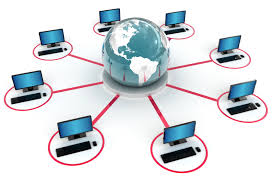
\includegraphics[width=10cm]{photos/cover.jpeg}
	\end{center}
\end{figure}

%	AUTHOR SECTION

\large
\begin{centering}
\end{centering}
{\begin{tabular}{lll}
\textsc{Legat} & Benoît & 4896 11 00\\
\textsc{Sedda} & Mélanie & 2246 11 00\\
\end{tabular}}
\\[1cm]

\normalsize
{\begin{tabular}{ll}
\textit{Teacher} : & Olivier Bonaventure\\
\textit{Assistants} : & Juan Antonio Cordero Fuertes\\
& Matthieu Baerts\\
& Raphael Bauduin\\
& David Lebrun\\
& Olivier Tilmans
\end{tabular}}
\\[1cm]

%	DATE SECTION

{\normalsize \today} % Date, change the \today to a set date if you want to be precise

\newpage

\end{titlepage}

%--------------------------------------------------------------------------
%	TABLE OF CONTENTS
%--------------------------------------------------------------------------
%
%\pagenumbering{gobble}
%\clearpage
%\thispagestyle{empty}
%\tableofcontents
%\clearpage
%\pagenumbering{arabic}

%--------------------------------------------------------------------------
%	CONTENT
%--------------------------------------------------------------------------

%--------------------------------------------------------------------------
%	IMPLEMENTATION CHOICES
%--------------------------------------------------------------------------
\section{Implementation choices}

\subsection{Sender}

We choose to create several agents responsible for different aspects of the sender and each running in a different thread so that these aspects can run in parallel.
\paragraph{Timer} This agent s responsible for everything related to the time. When another agent wants to launch an alarm that will expire at a certain time $t$, it delegates the work to the Timer. It sends it a message and the Timer will take care to prevent it once the time expired. This agent is useful both to implement the retransmission timer and to simulate the delays to send datas and receive acknowledgments.

Nous avons choisi de créer plusieurs agents chargés de différents aspects du sender et tournant chacun dans un thread différent pour que ces aspects distincts puissent s'exécuter en parallèle.
\paragraph{Timer} Cet agent qui se charge de tout ce qui concerne le temps. Quand un autre agent veut lancer une alarme qui expirera à un certain temps $t$, il délègue le travail au Timer. Il lui envoie un message et celui-ci se chargera de le prévenir une fois le délais écoulé. Le Timer est utile aussi bien pour implémenter les retransmission timer et que pour simuler les délais d'envoi des datas et de réception des acknowledgements.
\paragraph{Network Simulator} Cet agent est celui qui est réellement chargé de faire des \texttt{send()}.
\paragraph{Acker} Cet agent est celui qui fait les \texttt{recvfrom()}.
\paragraph{Selective repeat} Cet agent se charge de lire dans le fichier à envoyer et d'en faire des packets que le Network Simulator enverra. Il gère donc aussi la sending window. Il est tenu courant des acknowlegements reçus grâce au Acker, qui transmet l'information au Network Simulator, qui la fait parvenir au Selective Repeat.

\subsection{Receiver}
pas de recopiage dans buffer, joujou avec deux index

%--------------------------------------------------------------------------
%	LIMITATIONS
%--------------------------------------------------------------------------
\section{Limitations}

%--------------------------------------------------------------------------
%	PERFORMANCE
%--------------------------------------------------------------------------
\section{Factors limiting the performance}

%--------------------------------------------------------------------------
%	INTEROPERABILITY TEST
%--------------------------------------------------------------------------
\section{Interoperability test }

    
\end{document}